\chapter{Network Flow}

\section{Network Flow Problem}

\begin{itemize}
    \item \textbf{Input:}

    \begin{itemize}
        \item A direct graph $G = (V, E)$
        \item A capacity function $c: E \to \mathbb{R}_{\ge0}$
        \item The source $s \in V$ and the sink $t \in V$
    \end{itemize}

    \item \textbf{Output:} The maximum flow from $s$ to $t$
\end{itemize}

In a network flow problem, we assume
\begin{itemize}
    \item No edges enter $s$
    \item No edges leave $t$
    \item Edge capacity $c(e)$ is a non-negative integer
\end{itemize}

\begin{definition}[Flow]\index{Flow}\label{def:flow}
    An \term{$s-t$ flow} in a network is a function $f: E \to \mathbb{R}_{\ge 0}$ that satisfies the following properties:
    \begin{itemize}
        \item \textbf{Capacity constraint:} For all $e \in E$, \[ 0 \leq f(e) \leq c(e) \]
        \item \textbf{Flow conservation:} For all $v \in V \setminus \{s, t\}$, \[ \sum_{(v, u) \in E} f(v, u) = \sum_{(u, v) \in E} f(u, v) \]
    \end{itemize}

    Intuitively, $f(e)$ is the amount of flow that is sent through edge $e$.
\end{definition}

\begin{figure}[ht!]
    \centering
    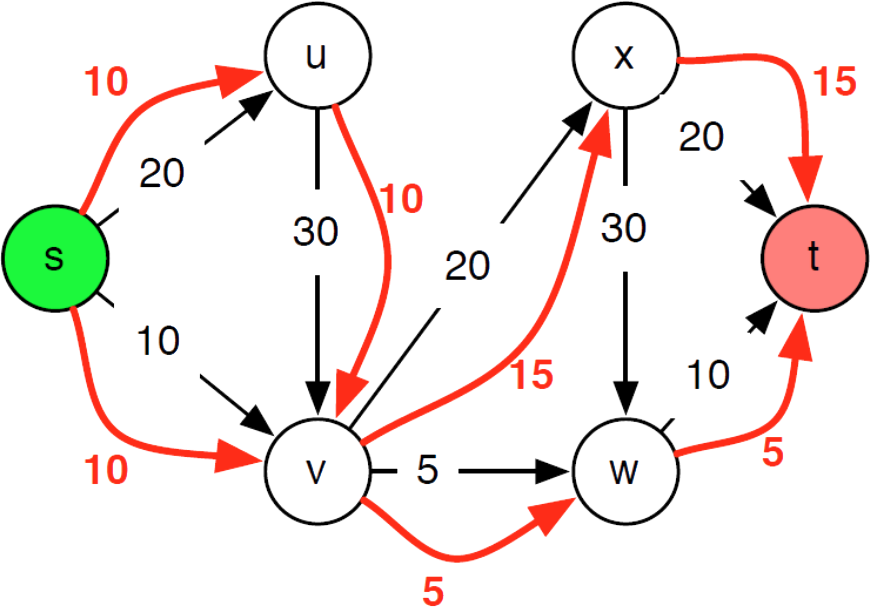
\includegraphics[width=0.33\linewidth]{figures/flow-definition.png}
\end{figure}

\begin{remark}[Notation]
    We define the function \[
        f^{in}(v) = \sum_{(u, v) \in E} f(u, v)
    \] to be the total flow into $v$, and \[
        f^{out}(v) = \sum_{(v, u) \in E} f(v, u)
    \] to be the total flow out of $v$.
\end{remark}

The value of the flow $f$ is defined as \[
    v(f) = f^{out}(s) = f^{in}(t)
\]

\begin{definition}[Network Flow Problem]\index{Network Flow Problem}\label{def:network-flow-problem}
    Given a network $G = (V, E)$, a capacity function $c: E \to \mathbb{R}_{\ge0}$, and two vertices $s, t \in V$, the \term{network flow problem} is to find an $s-t$ flow $f^*$ of maximum value.
\end{definition}

We can try to solve this problem using a greedy algorithm, but it doesn't always work -- once it increases the flow on an edge, it is not allowed to decrease it later. We need a way to ``undo'' the flow on an edge if it turns out to be a bad idea. To do so, we can send some flow \bred{backwards} along the same path.

\begin{figure}[ht!]
    \centering
    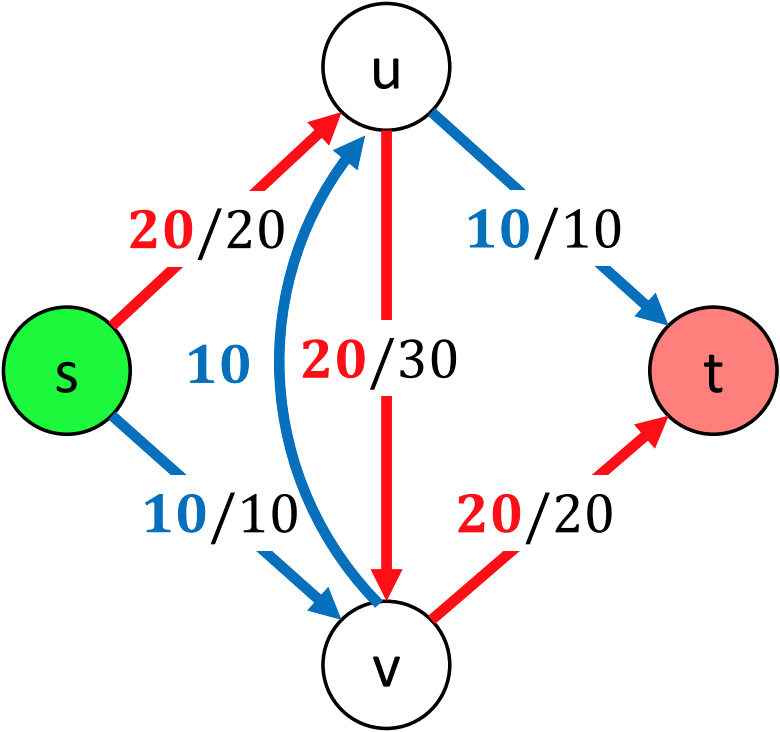
\includegraphics[width=0.25\linewidth]{figures/reverse-flow.png}
\end{figure}

\begin{definition}[Residual Graph]\index{Residual Graph}\label{def:residual-graph}
    Given a flow $f$ in a network $G = (V, E)$, the \term{residual graph} $G_f = (V, E_f)$ is a graph with the \bred{same vertices} as $G$, and edges $E_f$ defined as follows:
    \begin{itemize}
        \item \textbf{Forward edges:} $e = (u, v)$ with capacity $c(e) - f(e)$
        
        This is the amount of additional flow that can be sent along edge $e$.

        \item \textbf{Reverse edges:} $e^{rev} = (v, u)$ with capacity $f(e)$
        
        This is the amount of flow that can be sent backwards along edge $e$.
    \end{itemize}
\end{definition}

\begin{figure}[ht!]
    \centering
    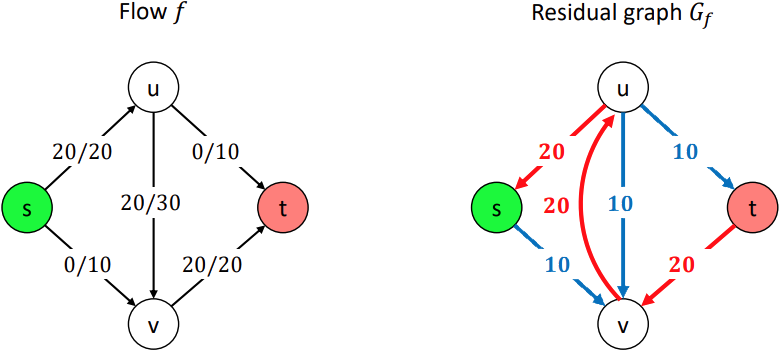
\includegraphics[width=0.63\linewidth]{figures/residual-graph.png}
\end{figure}

\begin{definition}[Augmenting Path]\index{Augmenting Path}\label{def:augmenting-path}
    Let $P$ be an $s-t$ path in the residual graph $G_f$. 

    Let $\text{bottleneck}(P, f)$ be the minimum capacity across all edges in $P$. 

    We \term{augment} flow $d$ by sending $\text{bottleneck}(P, f)$ units of flow along $P$. 

    \begin{itemize}
        \item For each forward edge $e \in P$, increase the flow on $e$ by $x$. 
        \item For each reverse edge $e^{rev} \in P$, decrease the flow on $e$ by $x$. 
    \end{itemize}
\end{definition}

\begin{figure}[ht!]
    \centering
    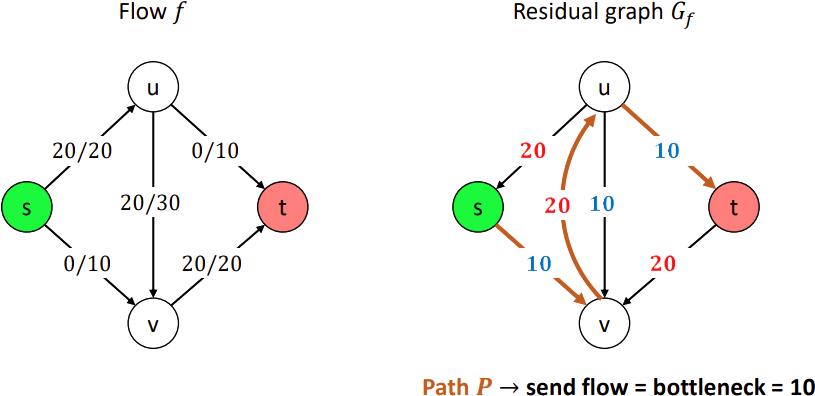
\includegraphics[width=0.65\linewidth]{figures/augmenting-path-1.png}
    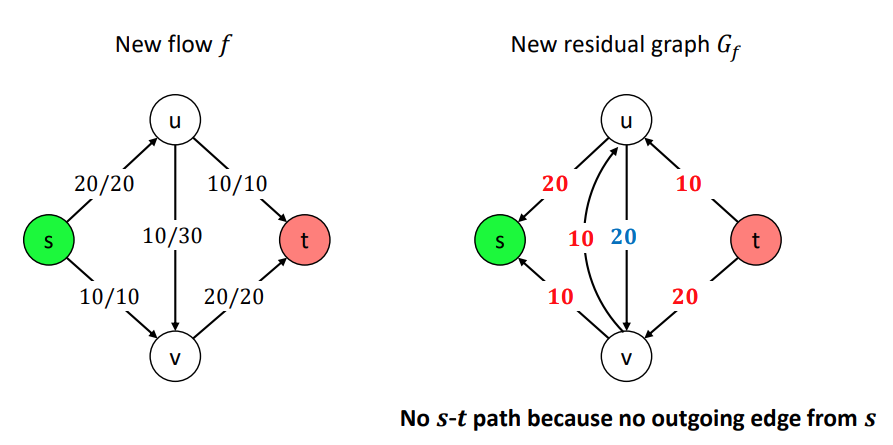
\includegraphics[width=0.65\linewidth]{figures/augmenting-path-2.png}
\end{figure}

We argue that the new flow is a valid flow. 

\begin{itemize}
    \item \textbf{Capacity constraint:} 
    
    \begin{itemize}
        \item If we \bred{increase} the flow on a forward edge, we can do so by \itblue{at most the capacity of forward edge} $e$ in $G_f$, which is $c(e) - f(e)$.
        
        So, the new flow can be at most $f(e) + \left( c(e) - f(e) \right) = c(e)$.

        \item If we \bred{decrease} the flow on a reverse edge, we can do so by \itblue{at most the capacity of reverse edge} $e^{rev}$ in $G_f$, which is $f(e)$.
        
        So, the new flow can be at most $f(e) - f(e) = 0$.
    \end{itemize}

    \item \textbf{Flow conservation:}

    Each node on the path (except $s$ and $t$) has exactly two incident edges. 

    \begin{center}
        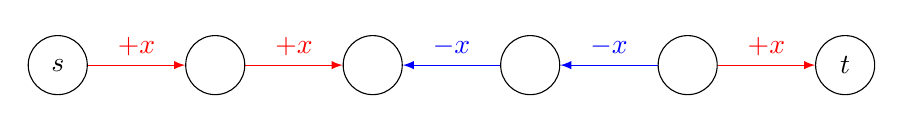
\begin{tikzpicture}
            \node[draw,circle,minimum size=0.75cm] (s) at (0, 0) {$s$};
            \node[draw,circle,minimum size=0.75cm] (1) at (2, 0) {};
            \node[draw,circle,minimum size=0.75cm] (2) at (4, 0) {};
            \node[draw,circle,minimum size=0.75cm] (3) at (6, 0) {};
            \node[draw,circle,minimum size=0.75cm] (4) at (8, 0) {};
            \node[draw,circle,minimum size=0.75cm] (t) at (10, 0) {$t$};

            \draw[-latex,red]  (s) -- (1) node[midway, above] {$+x$};
            \draw[-latex,red]  (1) -- (2) node[midway, above] {$+x$};
            \draw[-latex,blue] (3) -- (2) node[midway, above] {$-x$};
            \draw[-latex,blue] (4) -- (3) node[midway, above] {$-x$};
            \draw[-latex,red]  (4) -- (t) node[midway, above] {$+x$};
        \end{tikzpicture}
    \end{center}

    \begin{itemize}
        \item Both are forward / reverse edges. Then, one edge is incoming, and the other is outgoing.

        The flow is increased / decreased by the same amount.

        \begin{figure}[ht!]
            \centering
            \begin{subfigure}{0.45\linewidth}
                \centering
                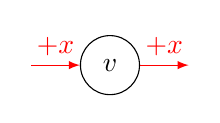
\begin{tikzpicture}
                    \node[draw,circle,minimum size=0.75cm] (v) at (0, 0) {$v$};

                    \draw[-latex,red] ++(180:1) -- (v)     node[midway, above] {$+x$};
                    \draw[-latex,red] (v)       -- ++(0:1) node[midway, above] {$+x$};
                \end{tikzpicture}

                \caption*{$f^{in}(v) \to +x \quad \text{and} \quad f^{out}(v) \to +x$}
            \end{subfigure}
            \hfil%
            \begin{subfigure}{0.45\linewidth}
                \centering
                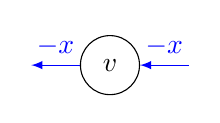
\begin{tikzpicture}
                    \node[draw,circle,minimum size=0.75cm] (v) at (0, 0) {$v$};

                    \draw[-latex,blue] (v)     -- ++(180:1) node[midway, above] {$-x$};
                    \draw[-latex,blue] ++(0:1) -- (v)       node[midway, above] {$-x$};
                \end{tikzpicture}

                \caption*{$f^{in}(v) \to -x \quad \text{and} \quad f^{out}(v) \to -x$}
            \end{subfigure}
        \end{figure}

        \item One forward, one reverse edge. Then, both edges are incoming or outgoing.

        The flow is increased on one edge and decreased on the other by the same amount.

        \begin{figure}[ht!]
            \begin{subfigure}{0.45\linewidth}
                \centering
                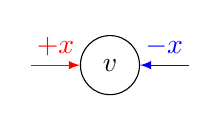
\begin{tikzpicture}
                    \node[draw,circle,minimum size=0.75cm] (v) at (0, 0) {$v$};

                    \draw[-latex,red]  ++(180:1) -- (v) node[midway, above] {$+x$};
                    \draw[-latex,blue] ++(0:1)   -- (v) node[midway, above] {$-x$};
                \end{tikzpicture}

                \caption*{$f^{in}(v)$ and $f^{out}(v)$ are unchanged}
            \end{subfigure}
            \hfil%
            \begin{subfigure}{0.45\linewidth}
                \centering
                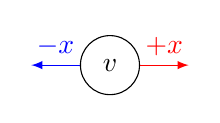
\begin{tikzpicture}
                    \node[draw,circle,minimum size=0.75cm] (v) at (0, 0) {$v$};

                    \draw[-latex,blue] (v) -- ++(180:1) node[midway, above] {$-x$};
                    \draw[-latex,red]  (v) -- ++(0:1)   node[midway, above] {$+x$};
                \end{tikzpicture}

                \caption*{$f^{in}(v)$ and $f^{out}(v)$ are unchanged}
            \end{subfigure}
        \end{figure}
    \end{itemize}
\end{itemize}

\section{Max Flow-Min Cut}

\subsection{Ford-Fulkerson Algorithm}

\begin{algorithm}[ht!]
    \begin{algorithmic}[1]
        \Function{Max-Flow}{$G$}
            \State {\color{gray} \texttt{// Initialize flow to 0:}}
            \State Set $f(e) = 0$ for all $e \in E$

            {~~~}

            \State {\color{gray} \texttt{// While there is an $s-t$ path in $G_f$:}}
            \While{$p = \Call{Find-Path}{s, t, \Call{Residual}{G,f}} \neq \texttt{None}$}
                \State $f \gets \Call{Augment}{f, p}$
                \State $\Call{Update-Residual}{G, f}$
            \EndWhile

            {~~~}

            \State \Return $f$
        \EndFunction
    \end{algorithmic}
\end{algorithm}

\subsubsection{Running Time Analysis}
\begin{itemize}
    \item \textbf{Number of Augmentations}
    
    \begin{itemize}
        \item At every step, flow and capacities remain integers. 
        \item For path $P$ in $G_f$, $\text{bottleneck}(P, f) > 0$ implies $\text{bottleneck}(P, f) \ge 1$.
        \item Each augmentation increases the flow by at least 1.
        \item The maximum flow (hence the number of augmentations) is at most $C = \sum_{e \text{ leaving } s} c(e)$.
    \end{itemize}

    \item \textbf{Preforming an Augmentation}
    
    \begin{itemize}
        \item $G_f$ has $n$ vertices and at most $2m$ edges. 
        \item Finding the path $P$, computing $\text{bottleneck}(P, f)$, and updating $G_f$ all take linear time. 
    \end{itemize}

    Thus, the running time of the Ford-Fulkerson algorithm is \[ O((m+n) \cdot C). \]
\end{itemize}

\subsubsection{Edmonds-Karp Algorithm}

This algorithm runs in \bred{pseudo-polynomial time} if we choose an \itblue{arbitrary} path in $G_f$ at each step. The value of $C$ can be exponentially larger in the input length (the number of bits requires to write down the edge capacities). 

\begin{example}
    In the graph below, we might end up repeatedly sending $1$ unit of flow across $a \to b$ and then reversing it. This takes $X$ steps, which can be exponential in the input length. 

    \begin{center}
        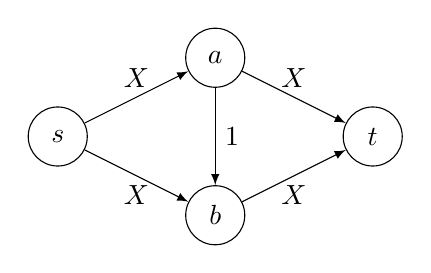
\begin{tikzpicture}
            \node[draw,circle,minimum size=0.75cm] (s) at (0, 0)  {$s$};
            \node[draw,circle,minimum size=0.75cm] (a) at (2, 1)  {$a$};
            \node[draw,circle,minimum size=0.75cm] (b) at (2, -1) {$b$};
            \node[draw,circle,minimum size=0.75cm] (t) at (4, 0)  {$t$};

            \draw[-latex] (s) -- (a) node[midway, above] {$X$};
            \draw[-latex] (s) -- (b) node[midway, below] {$X$};
            \draw[-latex] (a) -- (t) node[midway, above] {$X$};
            \draw[-latex] (b) -- (t) node[midway, below] {$X$};
            \draw[-latex] (a) -- (b) node[midway, right] {$1$};
        \end{tikzpicture}
    \end{center}
\end{example}

\begin{remark}[Pesudo-polynomial, Weakly Polynomial, and Strongly Polynomial]
    \begin{itemize}
        \item \textbf{Pseudo-polynomial time:} 
        
        The running time is polynomial in the unary representation of the input, \[
            ops = poly(m, n, X).
        \]

        \item \textbf{Weakly Polynomial time:} 
        
        The running time is polynomial in the binary representation of the input, \[
            ops = poly(m, n, \log X).
        \]

        \item \textbf{Strong polynomial time:} 
        
        The running time is polynomial in the input length, \[
            ops = poly(m, n).
        \]
    \end{itemize}
\end{remark}

To avoid the exponential running time, we need to be more careful about the path we choose. 

\begin{itemize}
    \item Find the \bred{maximum bottleneck capacity} augmenting path 
    
    This makes the algorithm run in \itblue{weakly polynomial time} \[
        \mathcal{O}(m^2 \cdot \log C)
    \]

    \item Find the \bred{shortest augmenting path} using BFS 
    
    This makes the algorithm run in \itblue{strongly polynomial time} \[
        \mathcal{O}(m^2 \cdot n).
    \] This is known as the \bred{Edmonds-Karp algorithm}\index{Edmonds-Karp Algorithm}.

    \begin{algorithm}[ht!]
        \begin{algorithmic}[1]
            \Function{Edmonds-Karp}{$G$}
                \State {\color{gray} \texttt{// Initialize flow to 0:}}
                \State Set $f(e) = 0$ for all $e \in E$

                {~~~}

                \State {\color{gray} \texttt{// Find shortest $s-t$ path in $G_f$:}}
                \While{$p = \Call{BFS}{s, t, \Call{Residual}{G,f}} \neq \texttt{None}$}
                    \State $f \gets \Call{Augment}{f, p}$
                    \State $\Call{Update-Residual}{G, f}$
                \EndWhile

                {~~~}

                \State \Return $f$
            \EndFunction
        \end{algorithmic}
    \end{algorithm}
    
    \begin{proof}
        Proof of \textsc{Edmonds-Karp} algorithm running time. 

        Let $d(v)$ be the distance from $s$ to $v$ in the residual graph $G_f$.

        \begin{lemma*}[1]\label{lem:edmonds-karp-1}
            During the execution of the algorithm, $d(v)$ does not decrease for any $v$.
        \end{lemma*}

        \begin{proof}(\hyperref[lem:edmonds-karp-1]{Lemma 1})

            Suppose augmentation $f \to f'$ decreases $d(v)$ for some $v$.

            Choose the $v$ with the smallest $d(v)$ in $G_{f'}$.

            Say $d(v) = k$ in $G_{f'}$, so $d(v) \ge k + 1$ in $G_f$.

            We look at node $u$ just before $v$ on a shortest path $s \to v \in G_{f'}$. 

            \begin{itemize}
                \item $d(u) = k - 1$ in $G_{f'}$
                \item $d(u)$ didn't decrease, so $d(u) \le k - 1$ in $G_f$.
            \end{itemize} 
            \[
                \begin{matrix}
                           & d(u)       & d(v)       \\
                    G_f    & \le k - 1  & \ge k + 1  \\
                           & \downarrow & \downarrow \\
                    G_{f'} & k - 1      & k
                \end{matrix}
            \]

            Then, in $G_f$, $(u, v)$ must be missing, as otherwise $d(v) \le d(u) + 1 = k$ in $G_f$.

            We must have added $(u, v)$ by selecting $(v, u)$ in augmenting path $P$.

            However, $P$ is a shortest path in $G_{f'}$, so it cannot have edge $(v, u)$ with $d(v) > d(u)$.
        \end{proof}

        We call edge $(u, v)$ \bred{critical} in an augmentation step if 
        \begin{itemize}
            \item It is part of the augmenting path $P$ and its capacity is equal to bottleneck$(P, f)$, or
            \item Augmentation step removes $e$ and adds $e^{rev}$ (if missing).
        \end{itemize}

        \begin{lemma*}[2]\label{lem:edmonds-karp-2}
            Between any two steps in which $(u, v)$ is critical, the distance $d(v)$ increases by at least 2.
        \end{lemma*}

        \begin{proof}(\hyperref[lem:edmonds-karp-2]{Lemma 2})
            
            Suppose $(u, v)$ was critical in $G_f$. The augmenting path must have removed it. 

            Let $k = d(u)$ in $G_f$. Since $(u, v)$ is part of a shortest path, $d(v) = k + 1$ in $G_f$.

            For $(u, v)$ to be critical again, it must be added back at some point. 
            \begin{itemize}
                \item Suppose $f' \to f''$ steps adds $(u, v)$ back.
                \item Augmenting path in $f'$ must have selected $(v, u)$.
                \item In $G_{f'}$, $d(v) = k + 1 \ge (k + 1) + 1 = k + 2$ by \hyperref[lem:edmonds-karp-1]{Lemma 1} on $v$.  \end{itemize}
        \end{proof}

        Each $d(u)$ can go from $0$ to $n$ by \hyperref[lem:edmonds-karp-1]{Lemma 1}.

        Then, each edge $(u, v)$ can be critical at most $\frac{n}{2}$ times by \hyperref[lem:edmonds-karp-2]{Lemme 2}.

        There can be at most $m \cdot \frac{n}{2}$ augmentation steps, and each augmentation takes $O(m)$ time.

        Thus, the running time of the Edmonds-Karp algorithm is \[
            O(m^2 \cdot n).
        \]
    \end{proof}
\end{itemize}

\subsection{Max Flow-Min Cut Theorem}

\begin{definition}[$s-t$ Cut]\index{$s-t$ Cut}\label{def:s-t-cut}
    An \term{$s-t$ cut} is a partition of the vertices $V = S \cup T$ such that $s \in S$ and $t \in T$.
\end{definition}

The capacity of an $s-t$ cut is the sum of the capacities of edges leaving $S$ and entering $T$ \[
    \text{cap}(S, T) = \sum_{u \in S} \sum_{v \in T} c(u, v)
\]

\begin{figure}[ht!]
    \centering
    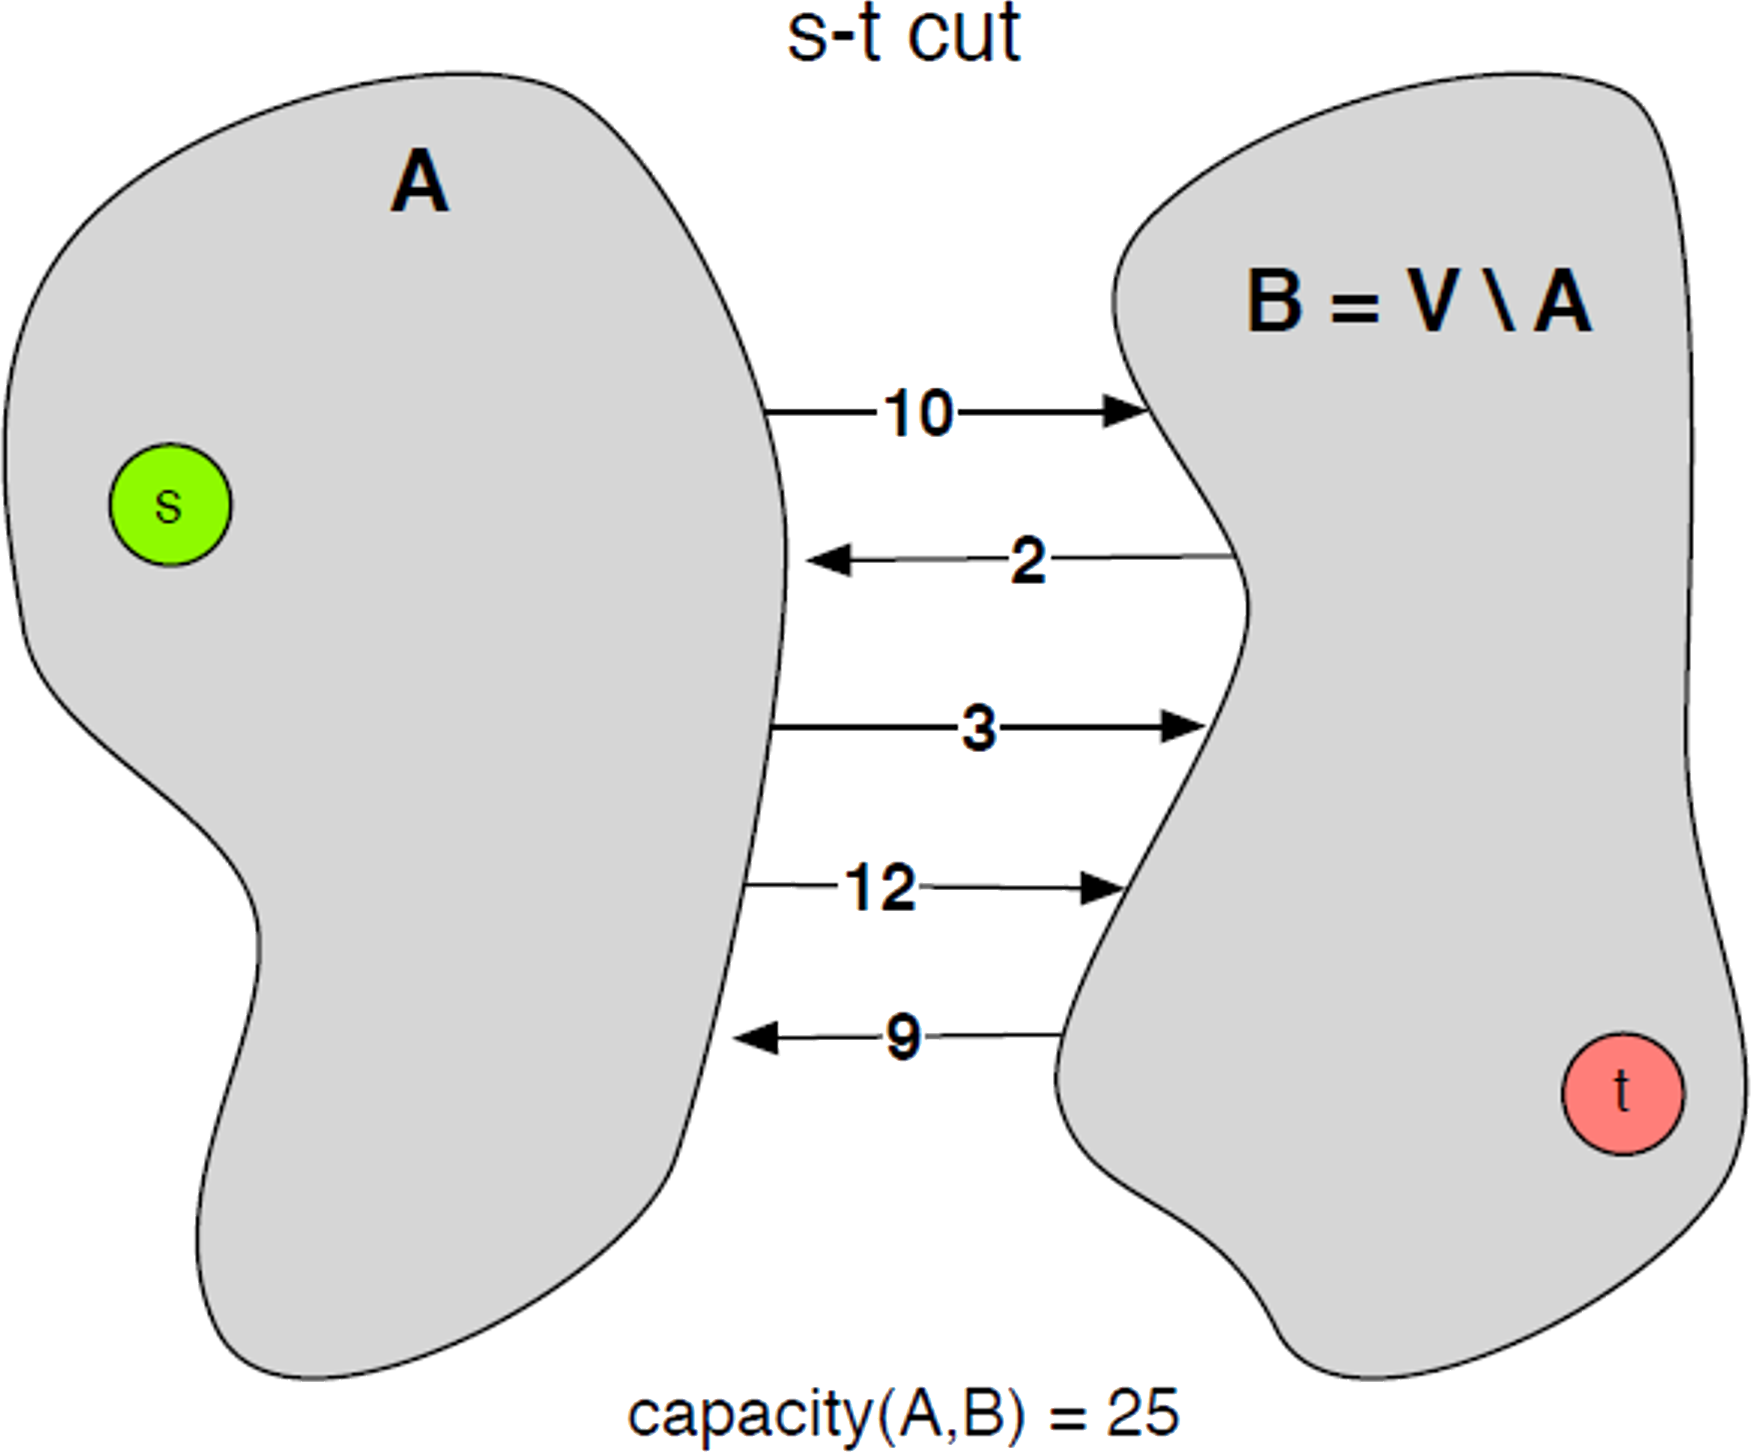
\includegraphics[width=0.33\linewidth]{figures/st-cut.png}
\end{figure}

\begin{theorem}
    For any flow $f$ and any $s-t$ cut $(S, T)$, \[
        v(f) = f^{out}(S) - f^{in}(S)
    \]
\end{theorem}

\begin{proof}
    Let $v \in S \setminus \{s\}$. Then,
    \begin{align*}
        f^{in}(v)
         & = f^{out}(v)                                                                     \\
        \sum_{v \in S \setminus \{s\}} \left( \sum_{e \text{ entering } v} f(e) \right)
         & = \sum_{v \in S \setminus \{s\}} \left( \sum_{e \text{ leaving } v} f(e) \right)
    \end{align*}

    After rearrangement, we get \[
        v(f) = f^{out}(S) - f^{in}(S)
    \]
\end{proof}

\begin{theorem}
    For any flow $f$, and any $s-t$ cut $(S, T)$, \[
        v(f) \le \text{cap}(S, T)
    \]
\end{theorem}

\begin{proof}
    \begin{align*}
        v(f) & = f^{out}(A) - f^{in}(A)             \\
             & \le f^{out}(A)                       \\
             & = \sum_{e \text{ leaving } A} f(e)   \\
             & \le \sum_{e \text{ leaving } A} c(e) \\
             & = \text{cap}(A, B)
    \end{align*}
\end{proof}

Hence, \[
    \max_{f} v(f) \le \min_{(S, T)} \text{cap}(S, T),
\] the maximum flow is at most the minimum cut.

\begin{theorem}
    Ford-Fulkerson algorithm finds a maximum flow $f^*$.
\end{theorem}

\begin{proof}
    WTS that the flow $f$ found by the Ford-Fulkerson algorithm is a maximum flow.

    Let $f$ be the flow found by the Ford-Fulkerson algorithm. 
    
    Let $G_f$ be the residual graph after the algorithm terminates.

    Let $A^*$ be the nodes reachable from $s$ in $G_f$, and let $B^* = V \setminus A^*$.

    \begin{center}
        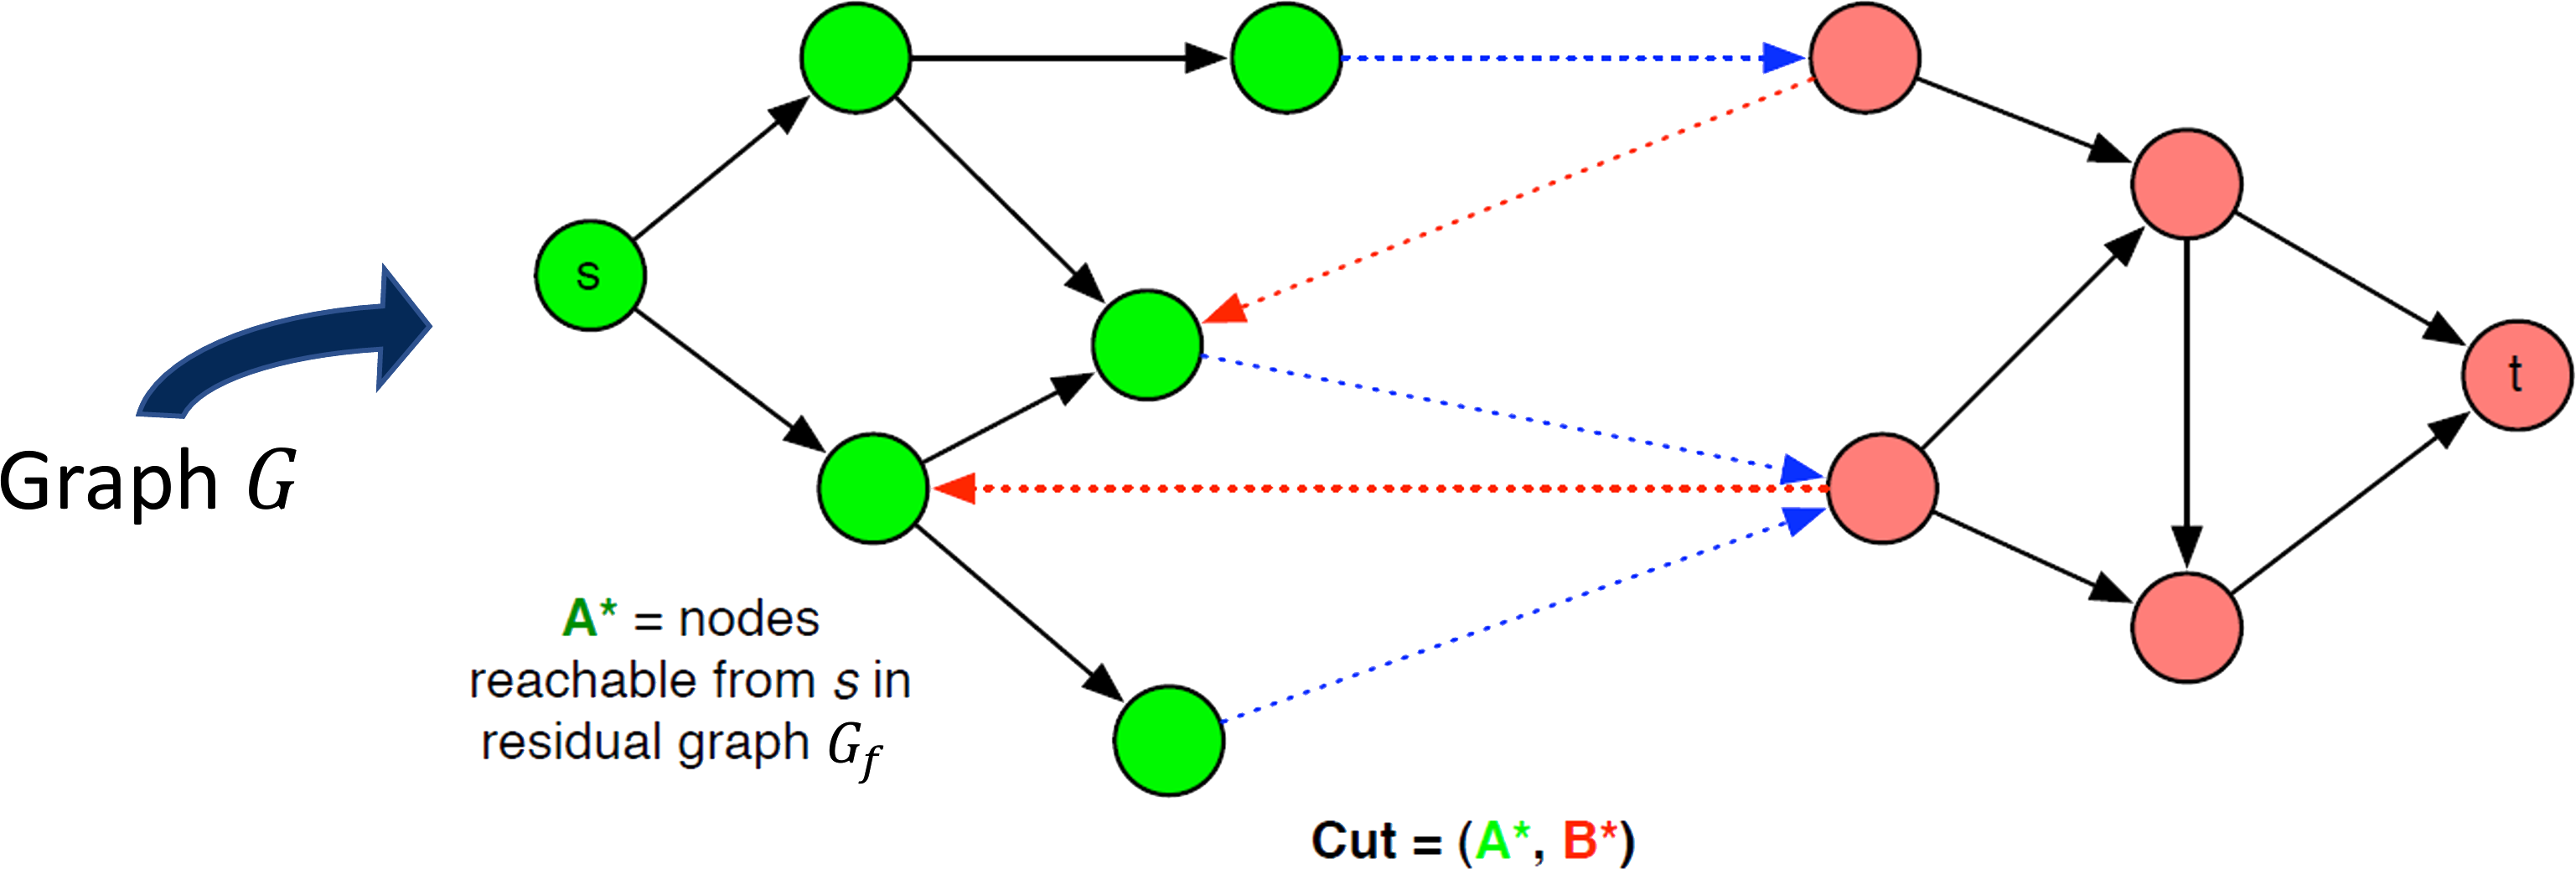
\includegraphics[width=0.67\linewidth]{figures/max-flow-min-cut.png}
    \end{center}

    \textbf{Claim:} $(A^*, B^*)$ is an $s-t$ cut.

    Indeed, $s \in A^*$ be definition. $t \in B^*$ because when Ford-Fulkerson terminates, there are no $s-t$ paths in $G_f$, so $s \notin A^*$. 

    {~~~}

    \begin{itemize}
        \item Let \blue{blue} edges be the edges going out of $A^*$ \bred{in $G$}, and 

        Each \blue{blue} edge $(u, v)$ must be saturated. 

        Otherwise, $G_f$ would have its forward edge $(u, v)$ and then $v \in A^*$. 

        Then, $f^{out}(A^*) = \text{cap}(A^*, B^*)$.

        \item Let \red{red} edges be the edges going out of $A^*$ \bred{in $G_f$}.

        Each \red{red} edge $(v, u)$ must have zero flow. 

        Otherwise, $G_f$ would have its reverse edge $(u, v)$ and then $v \in A^*$.

        Then, $f^{in}(A^*) = 0$.
    \end{itemize}

    Thus, \[
        v(f) = f^{out}(A^*) - f^{in}(A^*) = \text{cap}(A^*, B^*).
    \]
\end{proof}

\begin{theorem}[Max Flow-Min Cut Theorem]\index{Max Flow-Min Cut Theorem}
    In any flow network, the value of the maximum flow is equal to the capacity of the minimum cut.
\end{theorem}

\begin{proof}
    Run Ford-Fulkerson to find a max flow $f$. 

    Construct its residual graph $G_f$. 

    Le4t $A^*$ be the set of vertices reachable from $s$ in $G_f$.

    Then, $(A^*, V \setminus A^*)$ is a min $s-t$ cut.
\end{proof}

\section{Applications of Network Flow}

\subsection{Bipartite Matching}

\begin{definition}[Bipartite Graph]\index{Bipartite Graph}\label{def:bipartite-graph}
    A graph $G = (V, E)$ is \term{bipartite} if its vertex set $V$ can be partitioned into two sets $U$ and $V$ such that every edge in $E$ has one endpoint in $U$ and the other in $V$.
\end{definition}

A bipartite matching is when given a bipartite graph $G = (U \cup V, E)$, we want to find a maximum cardinality matching.

% TODO: Complete this section